\documentclass{article}

\usepackage{amsmath}
\usepackage{amssymb}
\usepackage{geometry}
\usepackage{fancyhdr}
\usepackage{graphicx}
\usepackage{array}
\usepackage{multirow}
\usepackage{tikz}
\usepackage{booktabs}
\usepackage{float}

\usetikzlibrary{calc,patterns,angles,quotes}




% for custom subsection
\usepackage{titlesec}
% package for enumerate with letters
\usepackage{enumitem}

\titleformat{\subsection}
  {\normalfont\fontfamily{phv}\fontsize{14}{17}}{\thesubsection}{1em}{}

\geometry{margin=1in}
\pagestyle{fancy}
\fancyhf{}
\rhead{Kyle Wodehouse}
\lhead{MSEG201}
\chead{Homework 2}
\title{\bfseries Homework 2}
\author{Kyle Wodehouse}
\rfoot{\thepage}
% 1 -> 5 from least to most descriptive
\setcounter{tocdepth}{1}

\begin{document}
\maketitle

\section{Unit Cell Volume}

For BCC the close packed direction is [111]. This can be visualized like this

% show picture chromium.png

\begin{figure}[H]
    \centering
    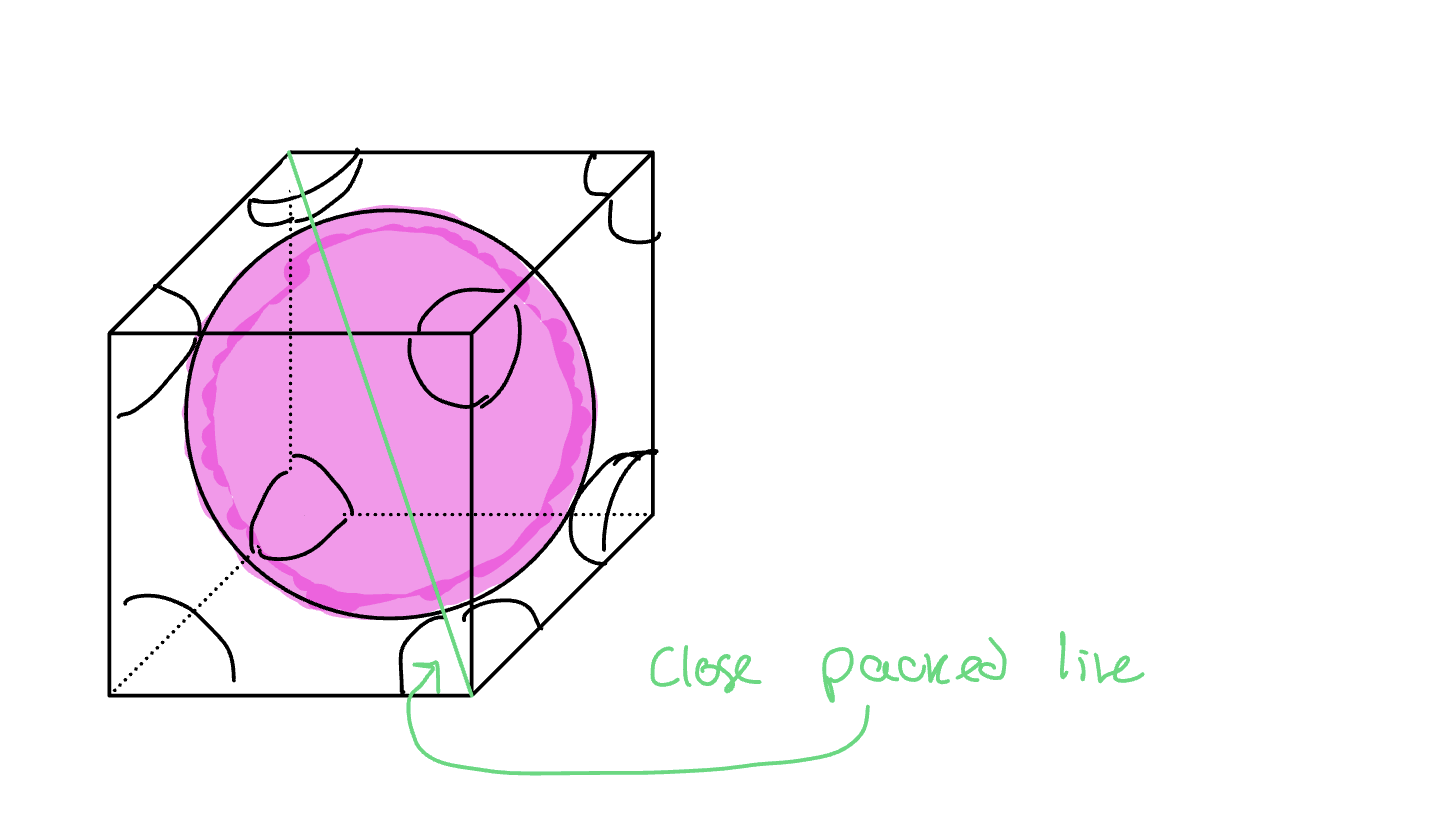
\includegraphics[width=0.7\textwidth]{chromium.png}
\end{figure}

Then looking at the geometry

% begin tickz picture

\begin{figure}[H]
    \centering
    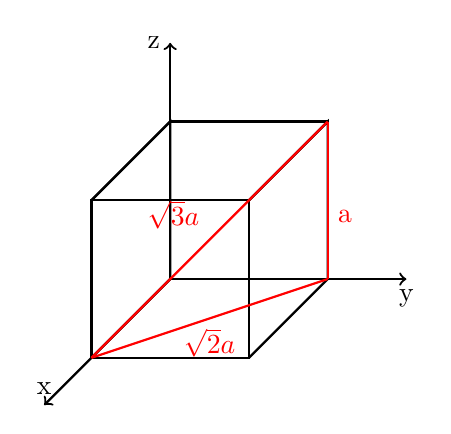
\begin{tikzpicture}
        \draw[thick, ->] (1,1) -- (1,4) node[anchor=east] {z};
        \draw[thick, ->] (1,1) -- (4,1) node[anchor=north] {y};
        \draw[thick, ->] (1,1) -- (-0.6,-0.6) node[anchor=south] {x};

        \draw[thick] (0,0) -- (0,2) -- (2,2) -- (2,0) -- (0,0);
        \draw[thick] (0,0) -- (1,1) -- (1,3) -- (0,2);
        \draw[thick] (2,0) -- (3,1) -- (3,3) -- (2,2);
        \draw[thick] (1,1) -- (3,1);
        \draw[thick] (1,3) -- (3,3);
        \draw[thick] (0,2) -- (1,3);
        \draw[thick] (2,2) -- (3,3);
        \draw[thick, red] (0,0) -- (3,1) node[midway, anchor=north] {$\sqrt{2} a$};
        \draw[thick, red] (3,1) -- (3,3) node[midway, anchor=north west] {a};
        \draw[thick, red] (0,0) -- (3,3) node[midway, anchor=south east] {$\sqrt{3} a$};
    \end{tikzpicture}
\end{figure}

Along this direction the atoms are touching, so the close packed direction also has 4 atomic radii

\begin{align*}
    4r &= \sqrt{3}a \\
    a &= \frac{4r}{\sqrt{3}} \\
    \vspace*{1em} \\
    V &= a^3 \\
    &= \left(\frac{4r}{\sqrt{3}}\right)^3 \\
    &= \left[ 0.1249 \textnormal{nm} \times \frac{4}{\sqrt{3}} \right]^{3} \\
    &= 0.02400 \textnormal{nm}^3
\end{align*}

\section{Planar Density}

\subsection*{(100) Plane}

\begin{figure}[H]
    \centering
    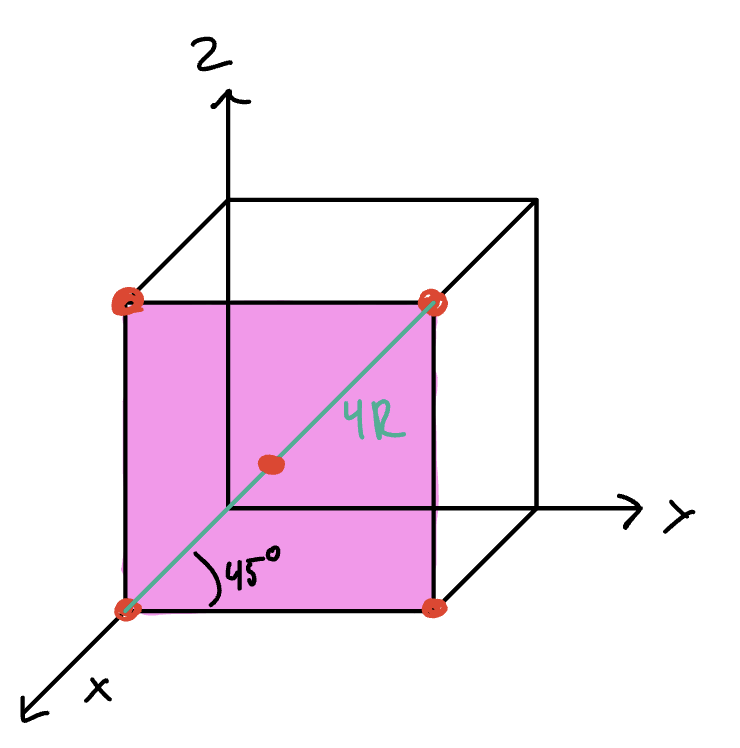
\includegraphics[width=0.5\textwidth]{100.png}
\end{figure}
\indent

From this we see the relationship between the lattice parameter and the atomic radius

\begin{align*}
    4r \cos(45^o) &= a \\
    a &= 2 \sqrt{2} r 
\end{align*}

And the area of the plane is 

\begin{align*}
    A &= a^2 \\
    &= (2 \sqrt{2} r)^2 \\
    &= 8r^2 \\
    &= 0.1242 \ \textnormal{nm}^2
\end{align*}

So the planar density is 

\[
    \frac{2}{0.1242} = 16 \ \textnormal{nm}^{-2}
\]

\subsection*{(110) Plane}

\begin{figure}[H]
    \centering
    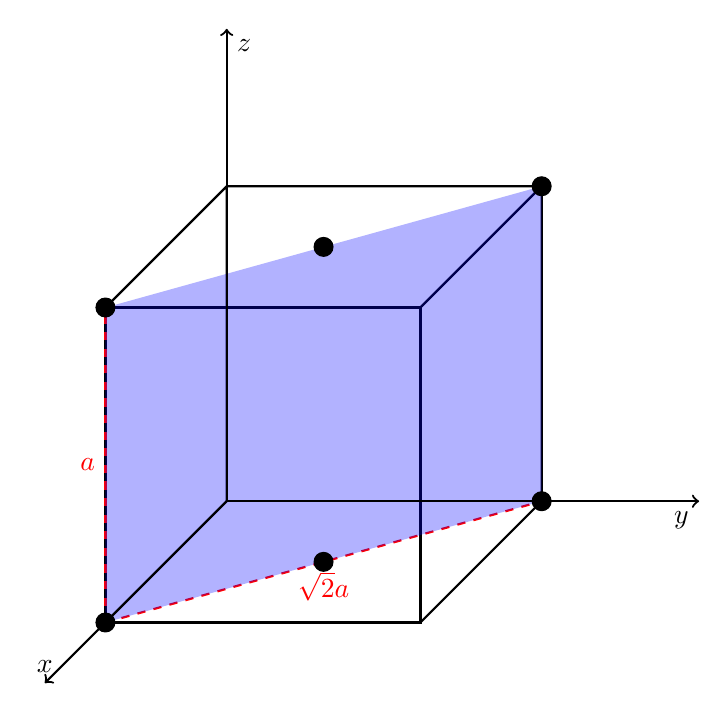
\begin{tikzpicture}[scale=4]
        % Draw the FCC unit cell
        \draw[thick] (0,0,0) -- (1,0,0) -- (1,1,0) -- (0,1,0) -- cycle; % Bottom face
        \draw[thick] (0,0,0) -- (0,0,1) -- (1,0,1) -- (1,0,0); % Front face
        \draw[thick] (0,0,0) -- (0,1,0) -- (0,1,1) -- (0,0,1); % Left face
        \draw[thick] (1,0,0) -- (1,1,0) -- (1,1,1) -- (1,0,1); % Right face
        \draw[thick] (0,1,0) -- (1,1,0) -- (1,1,1) -- (0,1,1); % Top face
        \draw[thick] (0,0,1) -- (1,0,1) -- (1,1,1) -- (0,1,1) -- cycle; % Back face

        % label a and \sqrt{2}a
        \draw[thick, dashed, red] (0,0,1) -- (1,0,0) node[midway, anchor=north] {$\sqrt{2} a$};
        \draw[thick, dashed, red] (0,0,1) -- (0,1,1) node[midway, anchor=east] {$a$};

        % Draw the (110) plane
        \fill[blue, opacity=0.3] (0,0,1) -- (1,0,0) -- (1,1,0) -- (0,1,1) -- cycle;

        % Label the axes
        \draw[thick, ->] (0,0,0) -- (1.5,0,0) node[anchor=north east] {$y$};
        \draw[thick, ->] (0,0,0) -- (0,1.5,0) node[anchor=north west] {$z$};
        \draw[thick, ->] (0,0,0) -- (0,0,1.5) node[anchor=south] {$x$};

        % put the atoms where they belong
            \filldraw[black] (0.5, 1, 0.5) circle (0.03cm);
            \filldraw[black] (0.5, 0, 0.5) circle (0.03cm);
            \filldraw[black] (0, 0, 1) circle (0.03cm);
            \filldraw[black] (0, 1, 1) circle (0.03cm);
            \filldraw[black] (1, 0, 0) circle (0.03cm);
            \filldraw[black] (1, 1, 0) circle (0.03cm);
        
        % Label the plane
        % \node at (0.5, 0.5, 0.5) [anchor=south] {$(110)$ Plane};
    \end{tikzpicture}
    \caption{(110) Plane in an FCC Unit Cell}
\end{figure}

The same relationship between $a$ and $r$, $a = 2\sqrt{2} \times r$, still holds. There are 2 half atoms and 4 quarter atoms in the plane, so there are two atoms in the plane. The diagonal of unit cell is $\sqrt{a}$, so 

\begin{align*}
    A &= a \times a \sqrt{2} \\
    &= 8 \sqrt{2} r^2 \\
    &= 0.1756 \textnormal{nm}^2
\end{align*}

So the planar density is 

\[
    \frac{2}{0.1756} = 11.4 \textnormal{nm}^{-2}
\]

\subsection*{(111) Plane}

\begin{figure}[H]
    \centering
    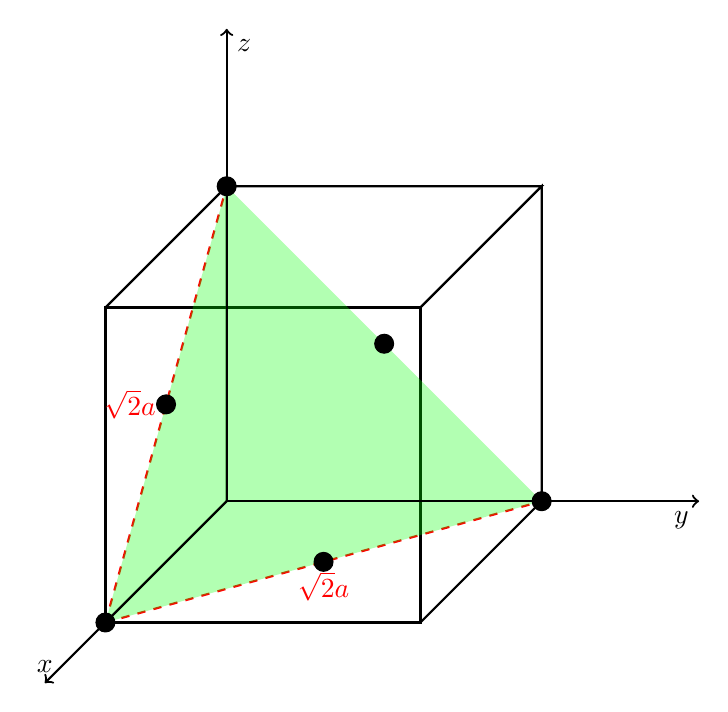
\begin{tikzpicture}[scale=4]
        % Draw the FCC unit cell
        \draw[thick] (0,0,0) -- (1,0,0) -- (1,1,0) -- (0,1,0) -- cycle; % Bottom face
        \draw[thick] (0,0,0) -- (0,0,1) -- (1,0,1) -- (1,0,0); % Front face
        \draw[thick] (0,0,0) -- (0,1,0) -- (0,1,1) -- (0,0,1); % Left face
        \draw[thick] (1,0,0) -- (1,1,0) -- (1,1,1) -- (1,0,1); % Right face
        \draw[thick] (0,1,0) -- (1,1,0) -- (1,1,1) -- (0,1,1); % Top face
        \draw[thick] (0,0,1) -- (1,0,1) -- (1,1,1) -- (0,1,1) -- cycle; % Back face

        % label a and \sqrt{2}a
        \draw[thick, dashed, red] (0,0,1) -- (1,0,0) node[midway, anchor=north] {$\sqrt{2} a$};
        \draw[thick, dashed, red] (0,0,1) -- (0,1,0) node[midway, anchor=east] {$\sqrt{2} a$};

        % Draw the (110) plane
        \fill[green, opacity=0.3] (0,0,1) -- (1,0,0) -- (1,0,0) -- (0,1,0) -- cycle;

        % Label the axes
        \draw[thick, ->] (0,0,0) -- (1.5,0,0) node[anchor=north east] {$y$};
        \draw[thick, ->] (0,0,0) -- (0,1.5,0) node[anchor=north west] {$z$};
        \draw[thick, ->] (0,0,0) -- (0,0,1.5) node[anchor=south] {$x$};

        % put the atoms where they belong
            \filldraw[black] (0, 0.5, 0.5) circle (0.03cm);
            \filldraw[black] (0.5, 0, 0.5) circle (0.03cm);
            \filldraw[black] (0, 0, 1) circle (0.03cm);
            \filldraw[black] (0.5, 0.5, 0) circle (0.03cm);
            \filldraw[black] (1, 0, 0) circle (0.03cm);
            \filldraw[black] (0, 1, 0) circle (0.03cm);

    \end{tikzpicture}
    \caption{(111) Plane in an FCC Unit Cell}
\end{figure}

The same relationship between $r$ and $a$ still holds. There are 3 half atoms and 3 1/6th atoms, so two atoms in the plane. For the area of the plane we can use the 

\begin{align*}
    A &= \frac{\sqrt{3}}{4} a^2 \\
    &= \frac{\sqrt{3}}{4} (\sqrt{2}(2\sqrt{2} r))^2 \\
    &= 4 \sqrt{3} r^2 \\
    &= 0.1075 \ \textnormal{nm}^2
\end{align*}

So the planar density is

\[
    \frac{2}{0.1075} = 18.6 \ \textnormal{nm}^{-2}
\]

\section{Theoretical Density}

From Table 12.3

\begin{table}[H]
    \centering
    \begin{tabular}{ c c }
        \hline
        Ion & Radius (nm) \\
        \hline
        $K^+$ & 0.138 \\
        $I^-$ & 0.220 \\
        \hline
    \end{tabular}
\end{table}

Which gives 

\[
    \frac{r_{K^+}}{r_{I^-}} = \frac{0.138}{0.220} = 0.627
\]

So this is predicted to be 6 coordinated, which is a rock salt structure. The theoretical density is

\begin{align*}
    \rho &= \frac{n' \times \left( A_c + A_n \right)}{V_c \times N_A} \\
    \tag*{(eqn 12.1 in the book)}
\end{align*}

$n'$ in this case is 4 because both of the ions are packed like FCC, which is 4 atoms per unit cell. $A_c$ is 39.098 in this case, and $A_n$ is 126.904. $V_c$ is the volume of the unit cell. Looking at just one of the faces of the unit cell

\begin{figure}[H]
    \centering
    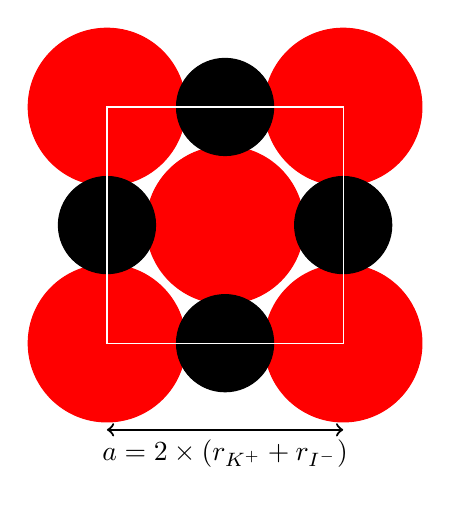
\begin{tikzpicture}

        \filldraw[red] (0,0) circle (1cm);
        \filldraw[red] (3,0) circle (1cm);
        \filldraw[red] (3,3) circle (1cm);
        \filldraw[red] (0,3) circle (1cm);
        \filldraw[red] (1.5,1.5) circle (1cm);

        \filldraw[black] (1.5,0) circle (0.617cm);
        \filldraw[black] (1.5,3) circle (0.617cm);
        \filldraw[black] (0,1.5) circle (0.617cm);
        \filldraw[black] (3,1.5) circle (0.617cm);

        \draw[white] (0,0) -- (3,0) -- (3,3) -- (0,3) -- cycle;

        \draw[thick, black, <->] (0,-1.1) -- (3,-1.1) node[midway, anchor=north] {$a = 2\times(r_{K^+} + r_{I^-})$};
    \end{tikzpicture}
\end{figure}

So the volume of the unit cell is

\begin{align*}
    V_c &= a^3 \\
    &= (2 \times (0.138 + 0.220))^3 \\
    &= 0.367 \ \textnormal{nm}^3 \times \left( \frac{1 \ \textnormal{cm}}{10^7 \ \textnormal{nm}} \right)^3
    &= 3.67 \times 10^{-23} \ \textnormal{cm}^3
\end{align*}

So, finally, the density is 

\begin{align*}
    \rho &= \frac{4 \times (39.098 + 126.904)}{3.67 \times 10^{-23} \times 6.022 \times 10^{23}} \\
    &= 3.01 \ \textnormal{g/cm}^3
\end{align*}

\section{X-ray Diffraction}

Replicating the figure Here

\begin{figure}[H]
    \centering
    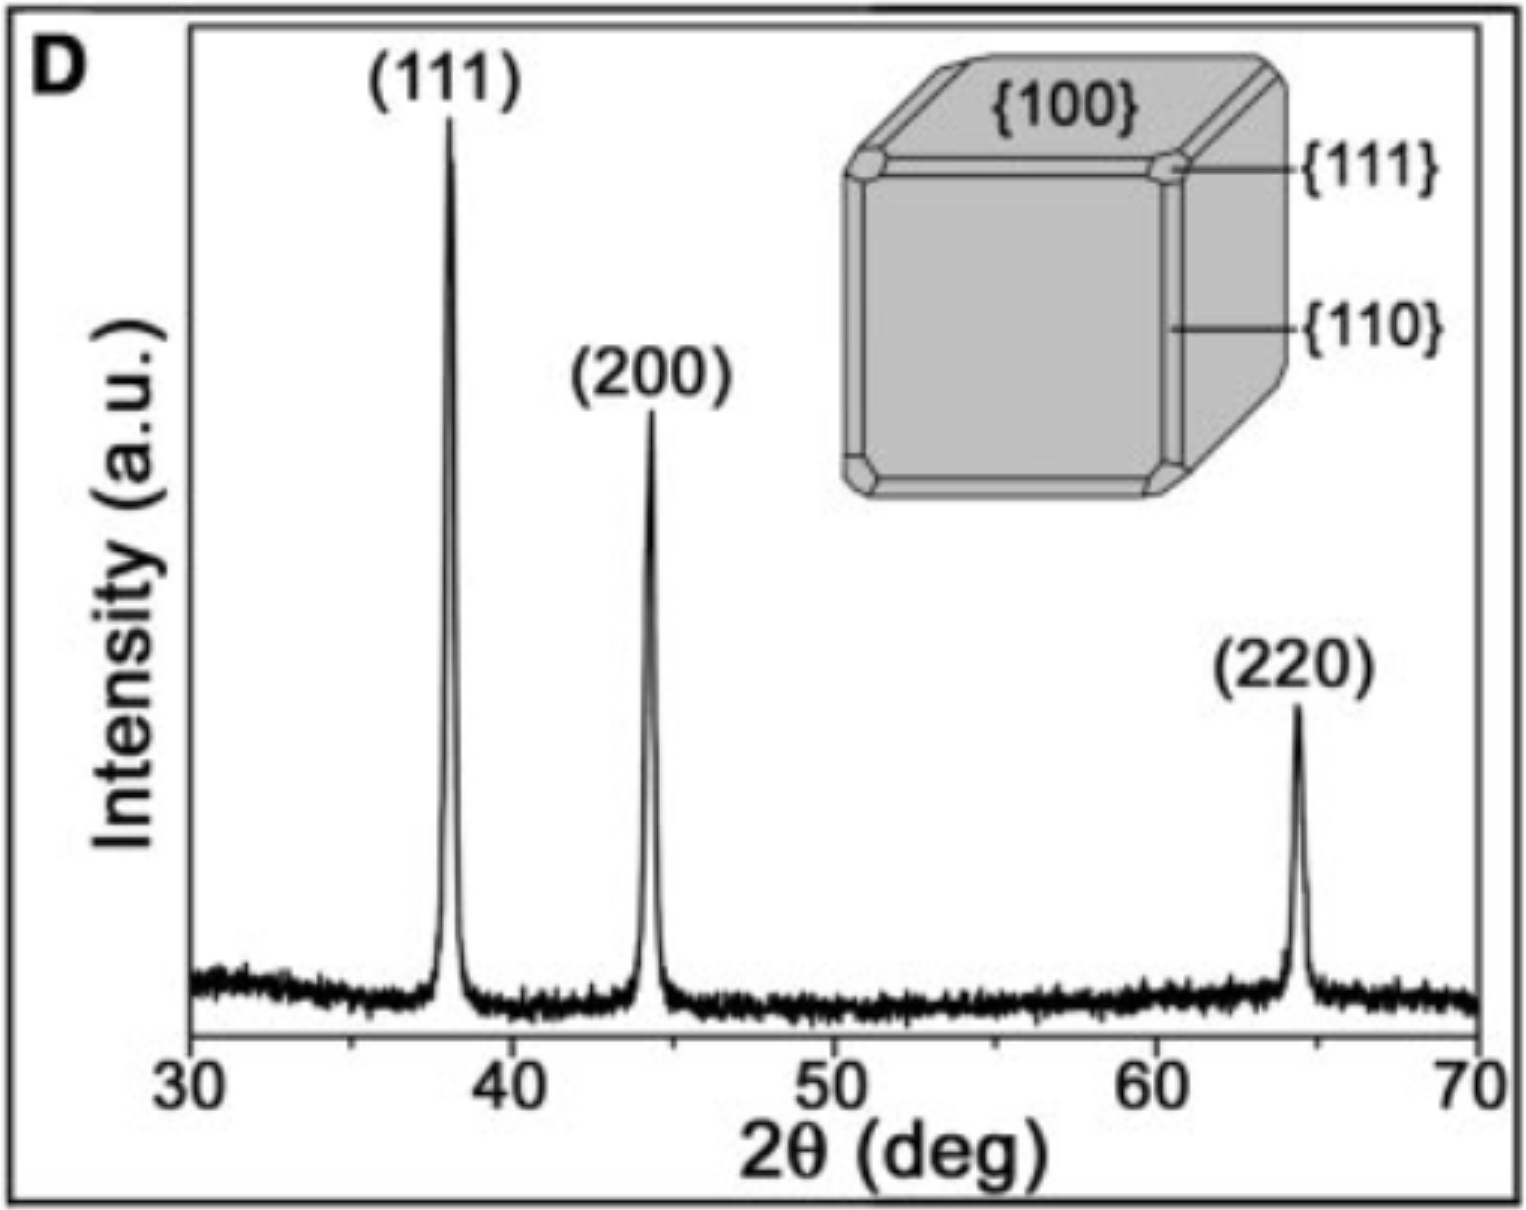
\includegraphics[width=0.5\textwidth]{1d.png}
\end{figure}

The authors say on the second page that they calculated the lattice constant, $a$, to be $4.088$ Angstromg. Looking at the (111) plane, \textit{assuming} that $n=1$, and reading the angle off the graph as $2 \theta = 38^o$,

\[
    d = \frac{a}{\sqrt{h^2 + k^2 + l^2}} = \frac{0.4088 \ \textnormal{nm}}{\sqrt{3}} = 0.2834 \ \textnormal{nm}
\]

\begin{align*}
    \lambda &= \frac{2 \cdot d \cdot \sin (\theta)}{n} \\
    \lambda &= \frac{2 \cdot 0.2834 \cdot \sin(\frac{38^o}{2})}{1} \\
    \lambda &= 0.154 \ \textnormal{nm}
\end{align*}

\section{X-ray Diffraction cont.}

\subsection*{a.}

Rearranging the Bragg equation and slapping in known values

\begin{align*}
    d &= \frac{n \cdot \lambda}{2\cdot\sin(\theta)} \\
    &= \frac{1 \cdot 0.0711}{2 \cdot \sin(\frac{20^o}{2})} \\
    &= 0.152 \ \textnormal{nm}
\end{align*}

\subsection*{b.}

We can use the d-spacing to find the lattice constant, and then that to find the radius

\begin{align*}
    d &= \frac{a}{\sqrt{h^2 + k^2 + l^2}} \\
    &= \frac{a}{\sqrt{3^2 + 2^2 + 1^2}} \\
    &= \frac{a}{\sqrt{14}} \\
    a &= d \cdot \sqrt{14} \\
    &= 0.152 \cdot \sqrt{14} \\
    &= 0.5698 \ \textnormal{nm}
\end{align*}

Then looking at a BCC unit cell


\begin{figure}[H]
    \centering
    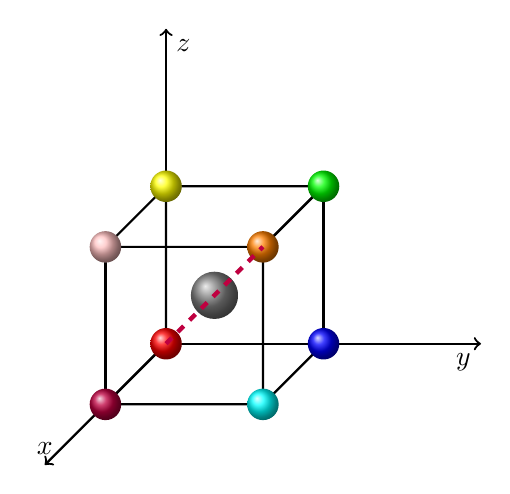
\begin{tikzpicture}[scale=2]
        % Draw the edges of the BCC unit cell
        \draw[thick] (0,0,0) -- (1,0,0) -- (1,1,0) -- (0,1,0) -- cycle; % Bottom face
        \draw[thick] (0,0,0) -- (0,0,1) -- (1,0,1) -- (1,0,0); % Front face
        \draw[thick] (0,0,0) -- (0,1,0) -- (0,1,1) -- (0,0,1); % Left face
        \draw[thick] (1,0,0) -- (1,1,0) -- (1,1,1) -- (1,0,1); % Right face
        \draw[thick] (0,1,0) -- (1,1,0) -- (1,1,1) -- (0,1,1); % Top face
        \draw[thick] (0,0,1) -- (1,0,1) -- (1,1,1) -- (0,1,1) -- cycle; % Back face

        \draw[thick,->] (0,0,0) -- (2,0,0) node[anchor=north east] {$y$};
        \draw[thick,->] (0,0,0) -- (0,2,0) node[anchor=north west] {$z$};
        \draw[thick,->] (0,0,0) -- (0,0,2) node[anchor=south] {$x$};

        % Draw the corner atoms
        \shade[ball color=red] (0,0,0) circle (0.1);
        \shade[ball color=blue] (1,0,0) circle (0.1);
        \shade[ball color=green] (1,1,0) circle (0.1);
        \shade[ball color=yellow] (0,1,0) circle (0.1);
        \shade[ball color=purple] (0,0,1) circle (0.1);
        \shade[ball color=cyan] (1,0,1) circle (0.1);
        \shade[ball color=orange] (1,1,1) circle (0.1);
        \shade[ball color=pink] (0,1,1) circle (0.1);
        \shade[ball color=gray] (0.5,0.5,0.5) circle (0.15);

        \draw[ultra thick, dashed, purple] (0,0,0) -- (1,1,1);
    \end{tikzpicture}
\end{figure}

The close packed direction is [111] (shown above in dashed line) and gives us the relationship

\begin{align*}
    4r &= \sqrt{3} \cdot a \\
    r &= \frac{\sqrt{3} \cdot a}{4} \\
    &= \frac{\sqrt{3} \cdot 0.5698 \ \textnormal{nm}}{4} \\
    &= 0.247 \ \textnormal{nm}
\end{align*}

\pagebreak

\section{HCP System}

\begin{figure}[H]
    \centering
    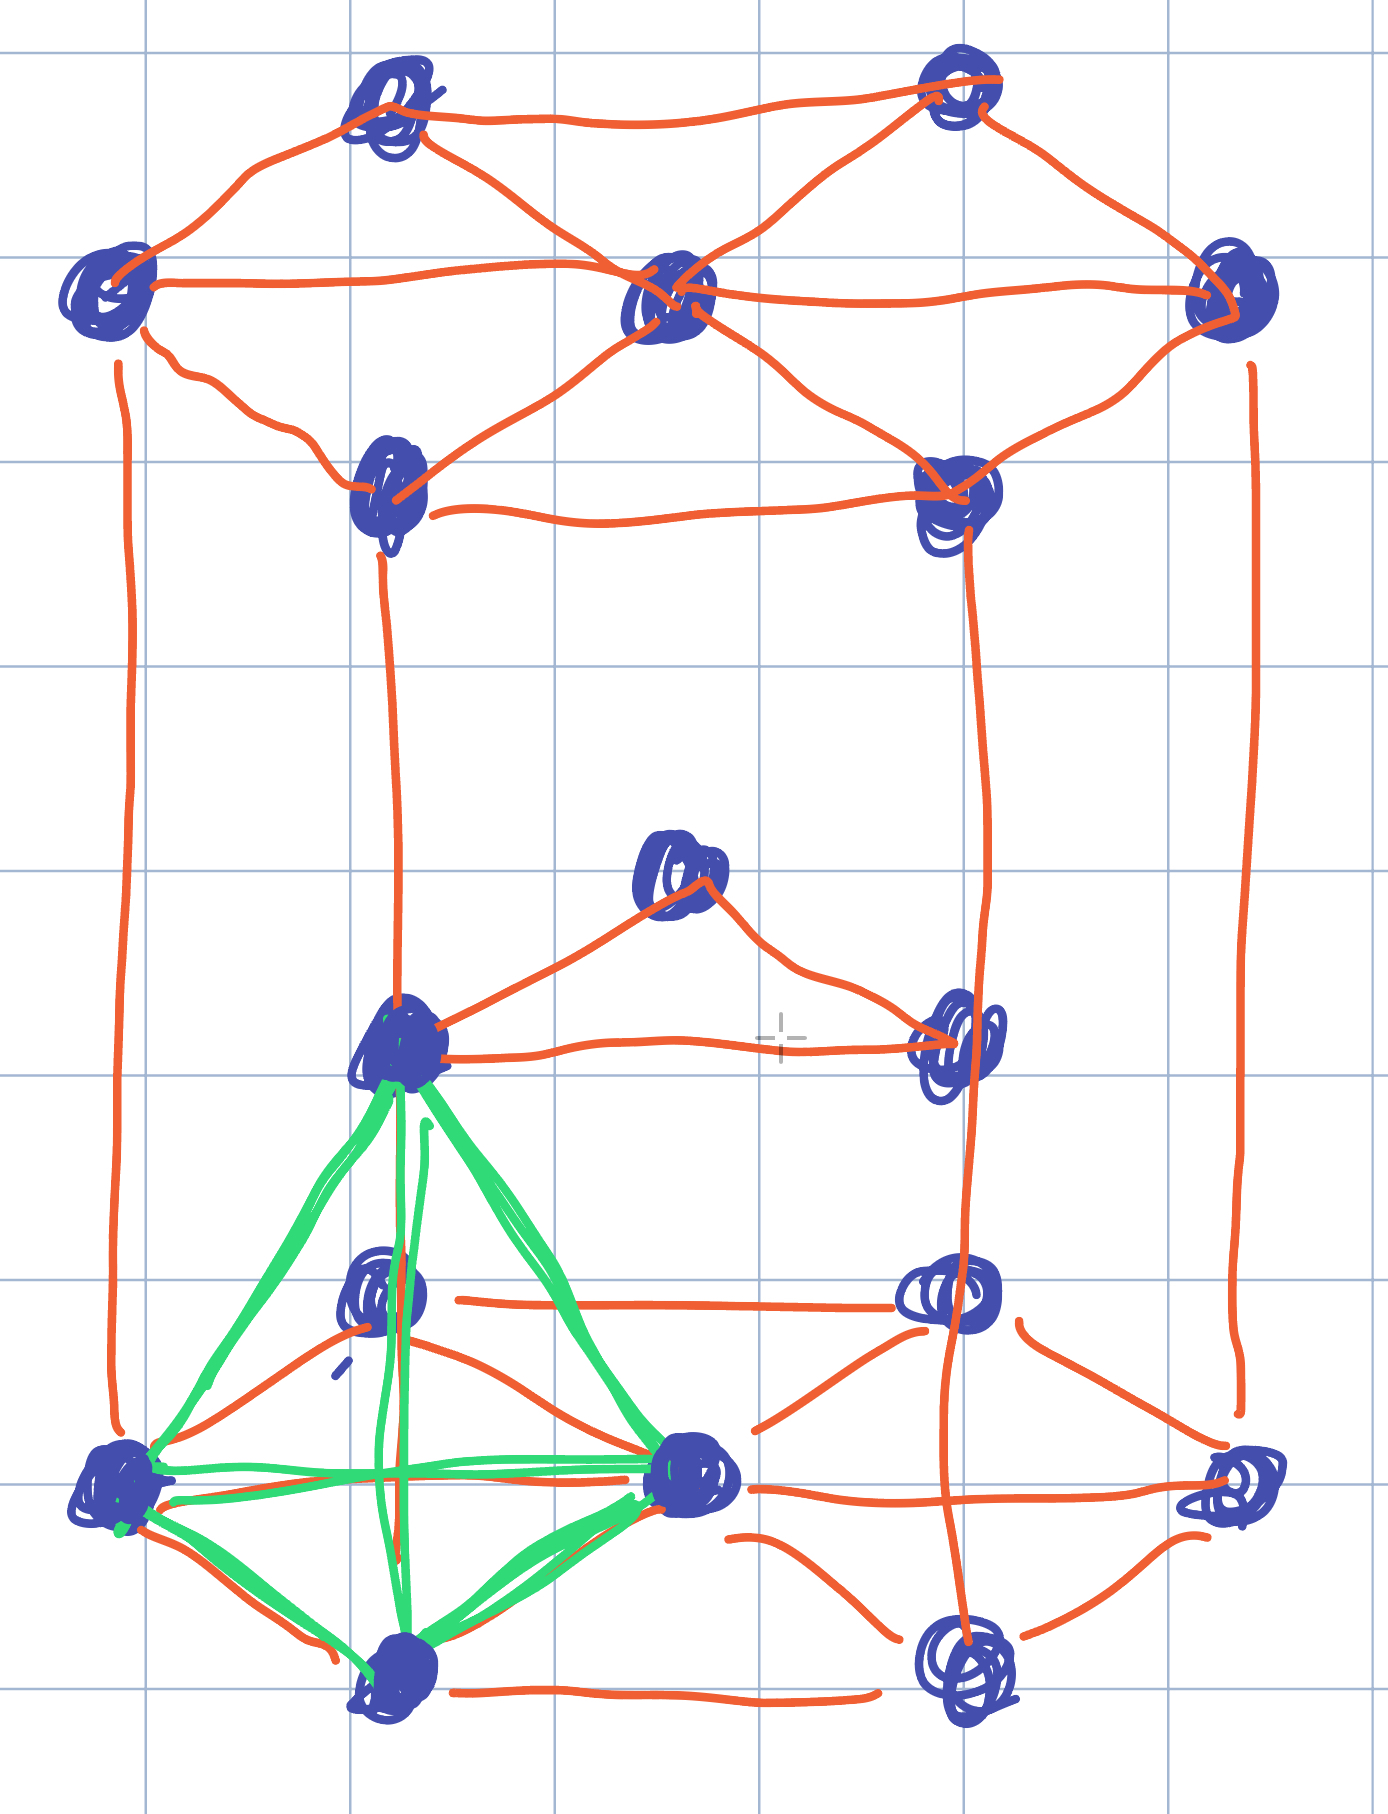
\includegraphics[width=0.3\textwidth]{hcp.jpeg}
\end{figure}

Looking at my little ipad sketch, you can see theres a fun tetrahedron I outlined in green. The tetrahedron has a height of $c/2$ and a base side length of $a$. The radius from the points of the base of the tetrahedron to the edges, $r$, can be visualized Here

\begin{figure}[H]
    \centering
    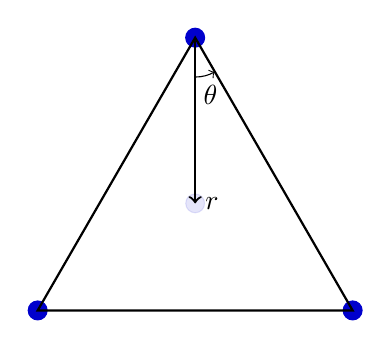
\begin{tikzpicture}[scale=4]
        \coordinate (1) at (0,0);
        \coordinate (2) at (1,0);
        \coordinate (3) at (0.5,0.866);
        \coordinate (4) at (0.5,0.34);

        \filldraw[blue!80!black] (1) circle (0.03cm);
        \filldraw[blue!80!black] (2) circle (0.03cm);
        \filldraw[blue!80!black] (3) circle (0.03cm);
        \filldraw[blue!80!black, opacity=0.1] (4) circle (0.03cm);

        \draw[thick] (0,0) -- (1,0) -- (0.5,0.866) -- cycle;
        \draw[thick, ->] (0.5,0.866) -- (0.5,0.34) node[anchor=west] {$r$};

        \pic [draw, ->, "$\theta$", angle eccentricity=1.5] {angle = 4--3--2};
    \end{tikzpicture}
\end{figure}

The angle $\theta$ is $30^o$, so

\begin{align*}
    \frac{a}{2} &= r \cos(30^o) \\
    r &= \frac{a}{\sqrt{3}}
\end{align*}

Delicious. Now Looking at another visualization of the tetrahedron

\begin{figure}[H]
    \centering
    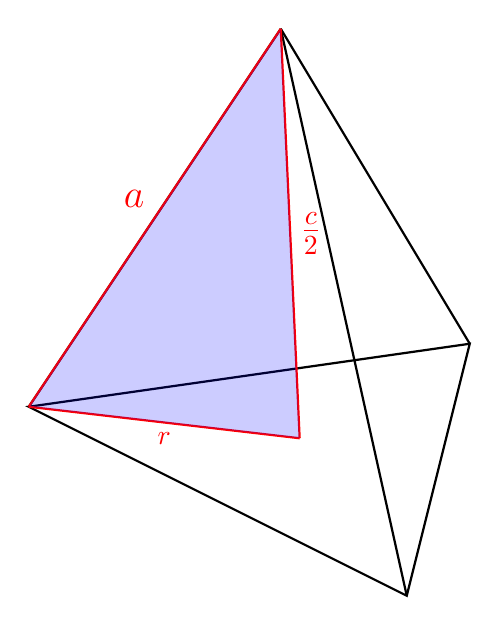
\begin{tikzpicture}[scale=0.8]
        \coordinate (1) at (0,0);
        \coordinate (2) at (7,1);
        \coordinate (3) at (6,-3);
        \coordinate (4) at (4,6);
        \coordinate (5) at (4.3,-0.5);

        \draw[thick] (1) -- (2) -- (3) -- cycle;
        \draw[thick] (1) -- (4);
        \draw[thick] (2) -- (4);
        \draw[thick] (3) -- (4);
        \draw[thick, red] (1) -- (5) node[midway, anchor=north] {$r$};
        \draw[thick, red] (5) -- (4) node[midway, anchor=west] {\Large$\frac{c}{2}$};
        \draw[thick, red] (1) -- (4) node[midway, anchor=south east] {\Large$a$};
        
        \fill[blue, opacity=0.2] (1) -- (5) -- (4) -- cycle;
    \end{tikzpicture}
\end{figure}

\begin{align*}
    a^2 &= \left( \frac{c}{2} \right)^2 + r^2 \\
    a^2 &= \left(\frac{a}{\sqrt{3}}\right)^2 + \left(\frac{c}{2}\right)^2 \\
    a^2 &= \frac{a^2}{3} + \frac{c^2}{4} \\
    \frac{2a^2}{3} &= \frac{c^2}{4} \\
    \frac{c^2}{a^2} &= \frac{8}{3} \\
    \frac{c}{a} &= \sqrt{\frac{8}{3}} \\
    &\approx 1.633
\end{align*}

\subsection{b.}

in each cell there are 12 1/6th atoms, 3 whole atoms, and 2 half atoms. So the number of atoms per cell is 6. The cell is close paced on the hexagon edges, so $2r = a$. We also know that $c = \sqrt{\frac{8}{3}} \cdot a$. 

The volume of the atoms is 

\[
    V_{atoms} = 6 \times \frac{4}{3} \pi r^3
\]

the volume of the unit cell is 

\begin{align*}
    V_{cell} &= c \times \left[ \frac{3\sqrt{3}}{2} a^2 \right] \\
    &= \left( 2 \sqrt{\frac{8}{3}} r \right)\left[ \frac{3\sqrt{3}}{2} (2r)^2 \right]
\end{align*}

So the pacing factor is 
\begin{align*}
    APF &= \frac{V_{atoms}}{V_{cell}} \\
    &= \frac{6 \times \frac{4}{3} \pi r^3}{\left( 2 \sqrt{\frac{8}{3}} r \right)\left[ \frac{3\sqrt{3}}{2} (2r)^2 \right]} \\
    &= \frac{\pi}{3 \sqrt{2}} \\
    &\approx 0.74
\end{align*}

And just to quick run through the math on the FCC in case I needed to show they're EXACTLY the same

\begin{figure}[H]
    \centering
    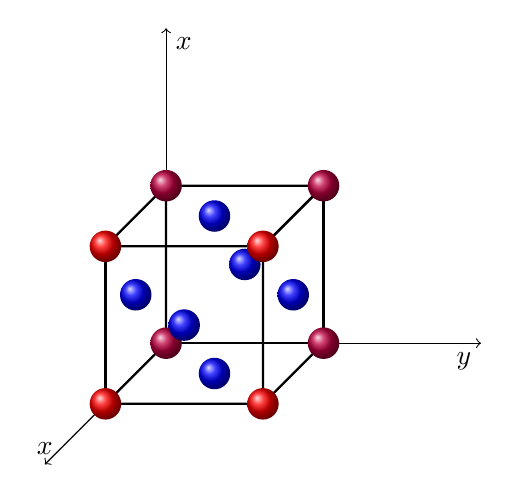
\begin{tikzpicture}[scale=2]
        \draw[->] (0,0,0) -- (2,0,0) node[anchor=north east] {$y$};
        \draw[->] (0,0,0) -- (0,2,0) node[anchor=north west] {$x$};
        \draw[->] (0,0,0) -- (0,0,2) node[anchor=south] {$x$};
        % Draw the edges of the FCC unit cell
        \draw[thick] (0,0,0) -- (1,0,0) -- (1,1,0) -- (0,1,0) -- cycle; % Bottom face
        \draw[thick] (0,0,0) -- (0,0,1) -- (1,0,1) -- (1,0,0); % Front face
        \draw[thick] (0,0,0) -- (0,1,0) -- (0,1,1) -- (0,0,1); % Left face
        \draw[thick] (1,0,0) -- (1,1,0) -- (1,1,1) -- (1,0,1); % Right face
        \draw[thick] (0,1,0) -- (1,1,0) -- (1,1,1) -- (0,1,1); % Top face
        \draw[thick] (0,0,1) -- (1,0,1) -- (1,1,1) -- (0,1,1) -- cycle; % Back face

        % Draw the corner atoms
        \shade[ball color=purple] (0,0,0) circle (0.1);
        \shade[ball color=purple] (1,0,0) circle (0.1);
        \shade[ball color=purple] (1,1,0) circle (0.1);
        \shade[ball color=purple] (0,1,0) circle (0.1);
        \shade[ball color=red] (0,0,1) circle (0.1);
        \shade[ball color=red] (1,0,1) circle (0.1);
        \shade[ball color=red] (0,1,1) circle (0.1);

        % Draw the face-centered atoms
        \shade[ball color=blue] (0.5,1,0.5) circle (0.1); % Front face
        \shade[ball color=blue] (0.5,0.5,0) circle (0.1); % Back face
        \shade[ball color=blue] (0.5,0.5,1) circle (0.1); % Left face
        \shade[ball color=blue] (1,0.5,0.5) circle (0.1); % Right face
        \shade[ball color=blue] (0.5,0,0.5) circle (0.1); % Bottom face
        \shade[ball color=blue] (0,0.5,0.5) circle (0.1); % Top face
        \shade[ball color=red] (1,1,1) circle (0.1);
    \end{tikzpicture}
    \caption{FCC Unit Cell with Blue Face-Centered Atoms and Red Corner Atoms}
\end{figure}

Of course the FCC has 4 atoms per cell, and the volume of the atoms is

\[
    V_{atoms} = 4 \times \frac{4}{3} \pi r^3
\]

We also know, in general, FCC has the relationship

\[
    4r = \sqrt{2} \cdot a
\]

So the volume of the unit cell is

\[
    V_{cell} = a^3 = \left( \frac{4r}{\sqrt{2}} \right)^3
\]

So the packing factor is

\begin{align*}
    APF &= \frac{V_{atoms}}{V_{cell}} \\
    &= \frac{4 \times \frac{4}{3} \pi r^3}{\left( \frac{4r}{\sqrt{2}} \right)^3} \\
    &= \frac{16\pi r^3}{\frac{32}{\sqrt{2}} r^3} \\
    &= \frac{2\sqrt{2}}{12} \pi \\
    &= \frac{\pi}{3\sqrt{2}} \\
    &\approx 0.74
\end{align*}

\end{document}